\chapter{Технологический раздел}

В данном разделе программирования, будут выбраны сконструированы среда разработки используемые классы, и а язык также спроектирован интерфейс программного продукта.

\section{Выбор и обоснование языка программирования и среды разработки}

В качестве языка программирования выбран язык C++, так как он обладает рядом преимуществ среди которых:
\begin{itemize}
	\item поддержка технологии объектно-ориентированного программирования, позволяющая:
	\begin{itemize}
		\item использовать наследование, полиморфизм и прочие возможности;
		\item представлять объекты сцены как объекты класса, что упростит организацию взаимодействия между ними и повысит читабельность;
		\item ускорить отрисовку сцены;
	\end{itemize}
	\item возможность использования широкого ряда шаблонов и библиотек;
	\item имеющийся опыт работы с ним в ранних курсах.
\end{itemize}

В качестве среды разработки выбран QtCreator, достоинствами которого являются:
\begin{itemize}
	\item простота в использовании;
	\item возможность создавать интерфейс и вести разработку внутри одного приложения;
	\item имеющийся опыт работы в данной среде.
\end{itemize}

\section{Структура и состав классов}

На рисунке \ref{classes_diagram} представлена диаграмма классов.

\begin{figure}[H]
	\begin{center}
		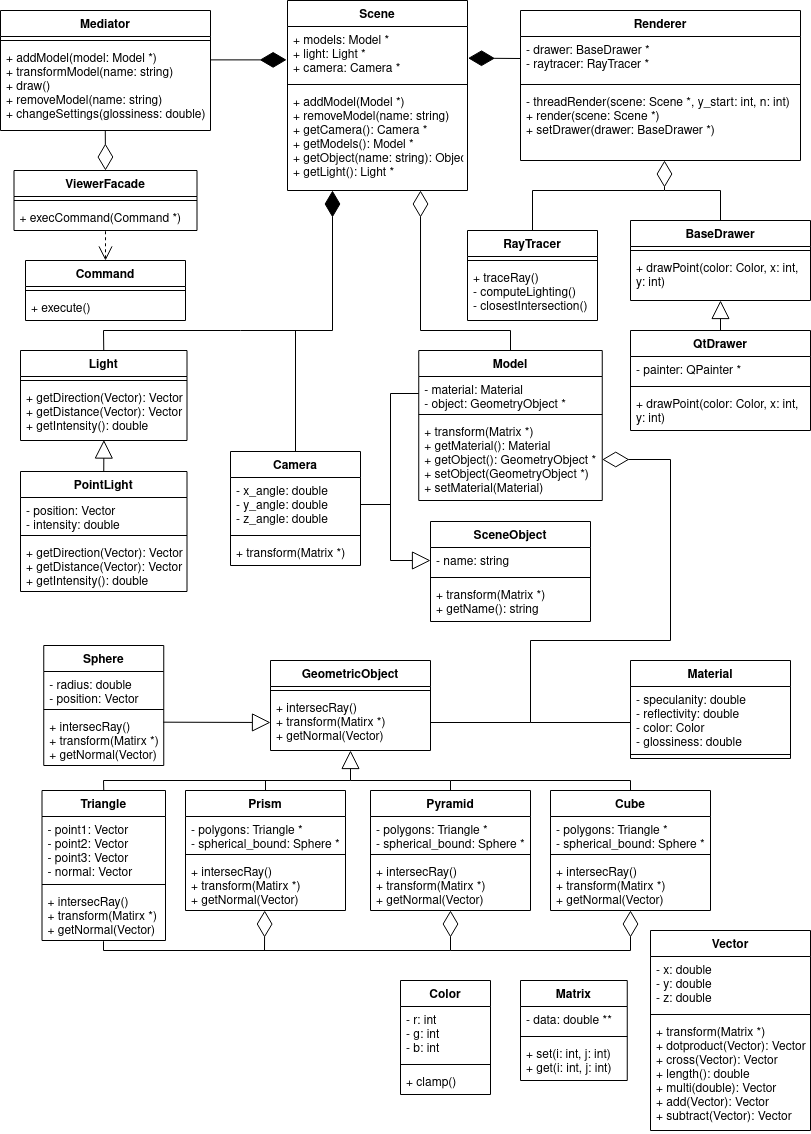
\includegraphics[scale=0.53]{assets/classes.png}
	\end{center}
	\caption{Диаграмма классов программы}
	\label{classes_diagram}
\end{figure}

Краткое описание классов:
\begin{itemize}
	\item ViewerFacade -- класс для взаимодействия пользовательского интерфейса и вычислительной части программы;
	\item Command -- абстракция команды пользовательского интерфейса, позволяет изолировать графический интерфейс от остальной программы;
	\item Mediator -- класс, упрощающий взаимодействие классов между собой, снижает межмодульную зависимость;
	\item Renderer -- класс для отрисовки изображения;
	\item BaseDrawer -- класс-обертка над QtDrawer, обеспечивает гибкую подмену используемых библиотек;
	\item RayTracer -- класс, реализующий алгоритм обратной трассировки лучей.
\end{itemize}

Для хранения информации о сцене и ее объектах были выделены следующие классы:
\begin{itemize}
	\item Scene -- класс, хранящий информацию о сцене;
	\item Light -- базовый класс источников света, позволит при необходимости добавлять различные типы источников освещения;
	\item PointLight -- класс точечного источника освещения;
	\item Camera -- класс, хранящий информацию о камере и позволяющий управлять ею;
	\item Model -- класс для хранения информации об объекте сцены;
	\item Material -- класс, хранящий информацию о материале объекта;
	\item Color -- класс, хранящий информацию о цвете объекта в формате RGB-тройки.
\end{itemize}

Также следует отдельно выделить математические классы:
\begin{itemize}
	\item GeometryObject -- базовый класс геометрических фигур, позволяет однообразно обрабатывать все типы геометрических объектов сцены;
	\item Sphere, Prism, Cube, Pyramid -- классы для представления конкретных геометрических объектов;
	\item Vector, Matrix, Triangle -- вспомогательные классы для упрощения работы с трехмерными объектами.
\end{itemize}

\section{Интерфейс программы}

На рисунке \ref{main_interface} представлено главное окно программы, содержащее следующие поля:
\begin{itemize}
	\item поля ввода для изменения координат и интенсивности источника света, которая может лежать в интервале от 0 до 1;
	\item поле ввода диффузной составляющей способности зеркала (неотрицательная величина);
	\item поля изменения направления и координат положения камеры;
	\item поле ввода количества лучей, обрабатываемых для отображения одного пикселя поверхности с коэффициентом диффузности отражения, отличным от 0.
\end{itemize}

\begin{figure}[H]
	\begin{center}
		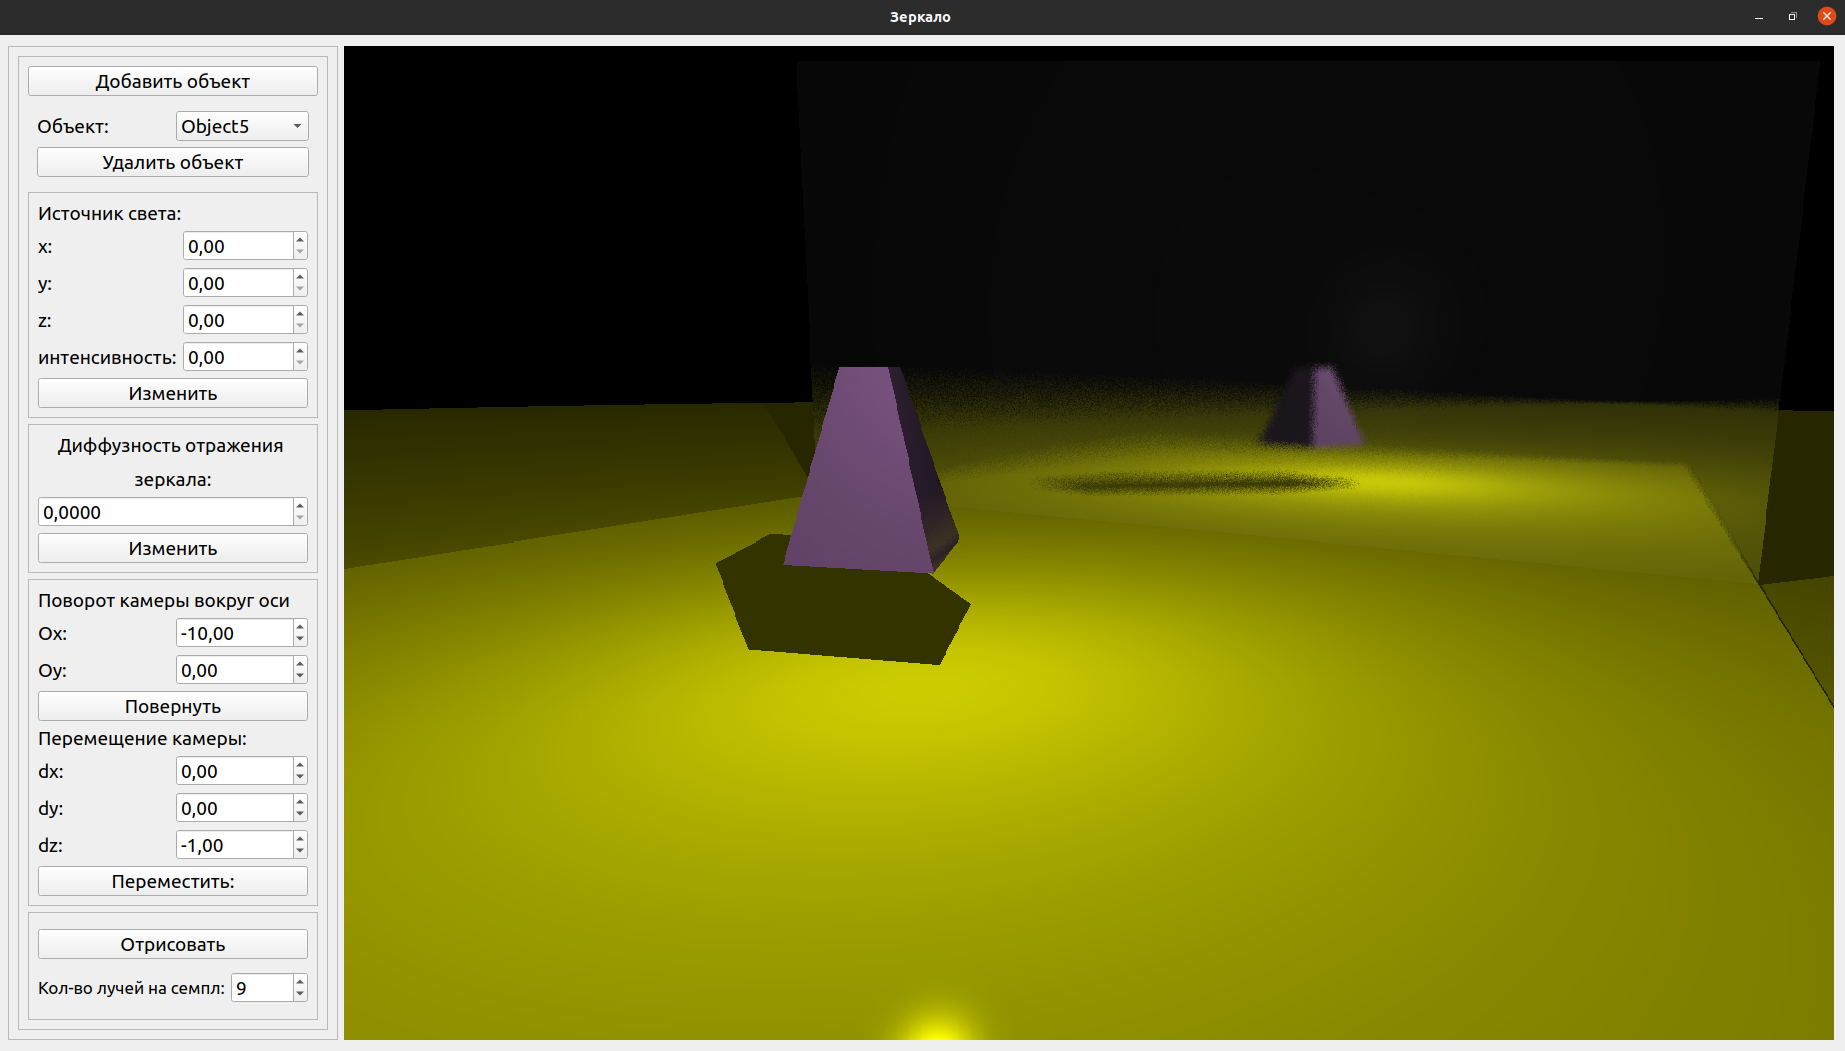
\includegraphics[scale=0.25]{assets/main_interface.png}
	\end{center}
	\caption{Интерфейс главного окна программы}
	\label{main_interface}
\end{figure}

Окна добавления геометрических объектов содержат следующие поля для ввода атрибутов:
\begin{itemize}
	\item сфера -- координаты центра и радиус;
	\item куб -- координаты левой нижней ближайшей вершины, длина ребра и угол поворота вокруг оси Oy;
	\item усеченная пирамида -- координаты левой нижней ближайшей вершины, длина основания, высота неусеченной версии пирамиды и высота усеченной (если исходная высота оказывается меньше усеченной, строится обычная четырехгранная пирамида высотой, равной наименьшему из двух значений), угол поворота вокруг оси Oy;
	\item призма -- координаты левой нижней ближайшей вершины, длина основания, высота призмы, угол поворота вокруг оси Oy.
\end{itemize}
Также каждое окно содержит поля для ввода свойств материала поверхности объектов: цвет, зеркальность, коэффициент отражения и шероховатость.

\newpage
На рисунке \ref{int2} представлено окно добавления куба.

\begin{figure}[H]
	\begin{center}
		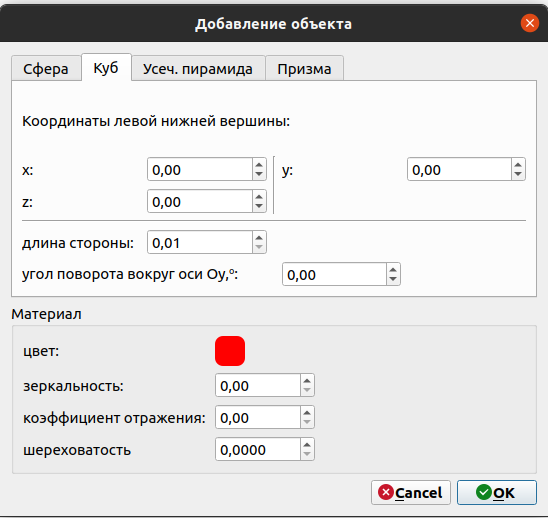
\includegraphics[scale=0.5]{assets/int2.png}
	\end{center}
	\caption{Окно добавления куба}
	\label{int2}
\end{figure}

\section{Вывод из раздела}

В данном разделе были выбраны язык программирования и среда разработки, разработана структура классов, а также интерфейс главного окна и окон добавления геометрических объектов.